\chapter{Introdução}

Escrever um trabalho científico pode ser uma tarefa desafiadora. \cite{severino}
destaca a complexidade e o rigor necessários na elaboração de trabalhos científicos, que não
apenas envolvem o domínio do conteúdo específico, mas também a aderência às normas
técnicas para apresentação formal e formatação correta.

A Associação Brasileira de Normas Técnicas 
(\acrshort{abnt})
, é a entidade responsável por,
dentre outras, fornecer as normas que regulam o processo de criação de trabalhos acadêmicos.
A Norma Brasileira Regulamentadora 
(\acrshort{nbr})
 Nº 14724, por exemplo: Especifica os princípios
gerais para a elaboração de (teses, dissertações e outros), visando sua apresentação à
instituição (banca, comissão examinadora de professores, especialistas designados e/ou
outros)
\cite{abnt}.

Ademais, ainda com respeito aos trabalhos acadêmicos, não somente a
regulamentação da 
\acrshort{nbr}
14724 deve ser observada. Há ainda a 
\acrshort{nbr}
6023 que trata a respeito
da elaboração de referências e a 
\acrshort{nbr}
10520, que diz respeito às citações em documentos.

\cite{castro}, adverte que: "Em ciência, não pode haver uma
separação entre forma e conteúdo. Trata-se de uma separação fictícia, pois fica se conhecendo
o conteúdo pela forma." Ou seja: A forma do trabalho, sua apresentação, sua formatação e
todo o seu arranjo gráfico é tão importante quanto seu conteúdo. 
\cite{medeiros} vai
complementar essa visão, afirmando que a apresentação gráfica "[...] contribui para a
consecução de um trabalho capaz de atingir seu objetivo. Monografia realizada sem a
preocupação gráfica, em geral, acaba malsucedida."

Em seu artigo, 
\cite{SilvaVitoria}
vão analisar as percepções e dificuldades dos
alunos de um curso superior em Tecnologia de Gestão em Recursos Humanos. Dentre suas
dificuldades, (dos alunos em questão), é destacada a questão da formatação do trabalho
acadêmico. Há também o fato de que as bancas avaliam os trabalhos baseadas em critérios da
própria Instituição de Ensino Superior (
\acrshort{ies}
), critérios estes que não estão necessariamente
presentes nas normas da \acrshort{abnt}, ou seja, há uma subjetividade presente que não é comum a
todas às \acrshort{ies} quanto a questão da formatação. Essa subjetividade contribui para a confusão dos
alunos, pois a \acrshort{ies} avaliará de acordo com aquilo que julga apropriado, o que muitas vezes
pode obscurecer o direcionamento do aluno ao redigir/formatar seu trabalho."

\clearpage

\cite{santos}
em seu Trabalho de Conclusão de Curso
(\acrshort{tcc})
, também analisa as
dificuldades encontradas por egressos, desta vez do curso de Ciências Contábeis da
Universidade Federal da Paraíba
(\acrshort{ufpb}).
Em sua pesquisa é destacado que "Quanto a
formatação do trabalho com as normas da 
\acrshort{abnt}, [...], 60\% teve alguma dificuldade, inclusive
32\% teve muita dificuldade.", ou seja, a formatação do trabalho é um grande desafio presente
na vida de boa parte dos estudantes em processo de escrita.

\section{Objetivo}

Levando em consideração os problemas que os alunos de diversas instituições de ensino enfrentam ao elaborar seus respectivos
trabalhos (conforme apresentado acima), o objetivo deste instrumento é desenvolver uma plataforma web de alta
interatividade\footnote{Refere-se à capacidade de um sistema, aplicação ou interface de responder
        às ações do usuário de maneira eficaz e intuitiva}
e
inteligibilidade\footnote{Refere-se à clareza e compreensibilidade da interface, documentação e feedback fornecidos pelo
    sistema. Um software inteligível facilita o entendimento do usuário sobre como utilizá-lo e quais são os resultados de suas ações.},
de modo que o discente possa se preocupar apenas com o conteúdo. Os detalhes de formatação, de acordo com os padrões da
\acrshort{abnt}
e da
\acrshort{ies},
ficarão a cargo da própria plataforma.

A criação de um trabalho de
\acrshort{tcc}
se dará basicamente por três passos básicos: Escrita em blocos;
\textit{Parsing}\footnote{O termo Parsing, (do inglês: análise), será utilizado no
sentido de analisar e transformar algo em outra coisa.}
e
Documento em
\acrshort{pdf}
. A Figura\ref{fig:Passos para criar um documento} ilustra esse fluxo na linha do tempo.

\begin{figure}[ht]
    \centering
    \caption{Passo a passo para criar um documento na plataforma}
    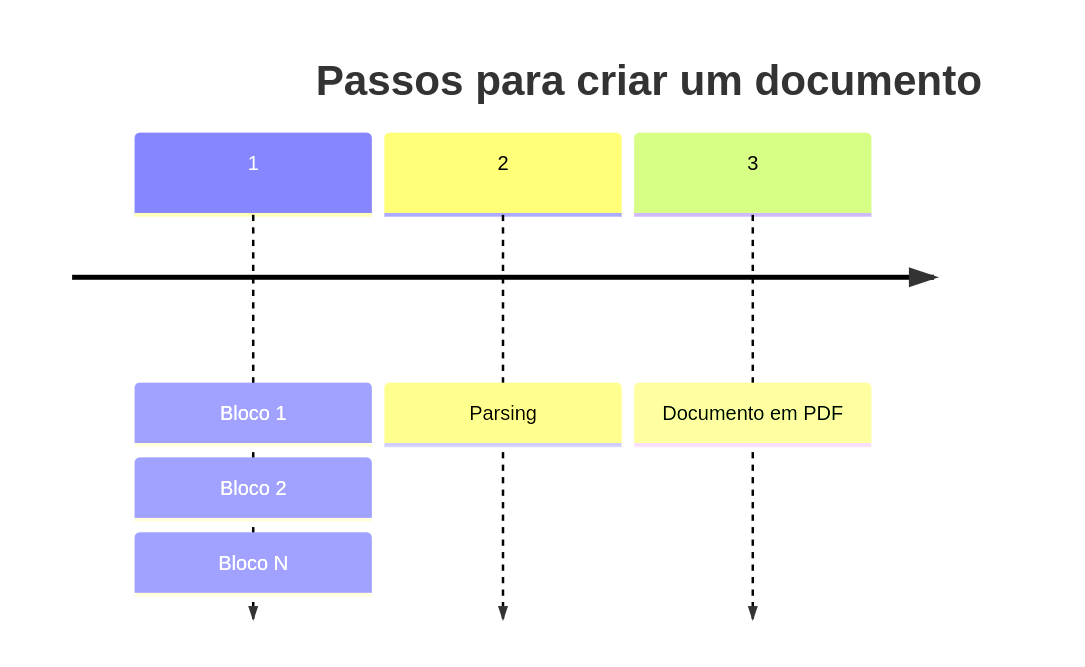
\includegraphics[width=0.8\textwidth]{./images/Passos para criar um documento.png}
    \label{fig:Passos para criar um documento} \\
    \textnormal{\fontsize{10pt}{12pt}Fonte: Autoria própria}
\end{figure}

O usuário interagirá com a aplicação escrevendo blocos que serão transformados
no documento final em
\acrshort{pdf}
. A este processo daremos o nome de Parsing. Após este, bastará
enviar o download do \acrshort{pdf}
ao usuário com todo o padrão de formatação. Os trabalhos desenvolvidos nesta plataforma
terão então duas versões: A versão de blocos, (sem formatação e interativa); e a versão
final já formatada em \acrshort{pdf}.

\section{Fluxo do documento}

\subsection{Escrita em blocos}

A escrita se dará de modo em que tudo será considerado um bloco.
A escrita em blocos consiste numa abordagem em que o texto vai sendo
escrito em seu fluxo natural, porém blocos podem ser adicionados à escrita.
Um bloco é um elemento adicionado ao fluxo de trabalho que desenpenha um papel
que o diferencia dos demais blocos.
Por exemplo: Uma imagem pode ser considerada um bloco nesta abordagem, uma vez
que não é um texto mas tem o objetivo de fornecer informações visuais. O próprio corpo
do texto em si será considerado um bloco, denominado parágrafo. Um título será um bloco
textual cujo objetivo será separar sessões do texto coesas. Uma lista será um bloco para enumerar
intens e assim por diante. O documento será basicamente uma composição de diversos blocos dispostos de forma a formar
uma unidade coesa final, que será o trabalho propiamente dito.

\subsection{Bloco}

Um bloco é uma unidade lógica no documento que desenpenha um papel especializado que nenhum
outro bloco o faz. Por exemplo: O bloco mais importante da
plataforma\footnote{O termo plataforma será utilizado
    de forma intercambiável e como sinônimo de aplicativo; sistema web; ou aplicativo da web}
será o de texto, (denominado bloco parágrafo), pois sem texto, não há trabalho.
Sem texto não há tão pouco comunicação que transmita informação
de caráter acadêmico-científico.

Semelhante ao bloco de texto, diversos outros blocos adjascentes
auxiliarão na construção do documento acadêmico. O bloco de imagem, por
exemplo, ajuda a exibir informações de forma ilustrativa e auxilia bastante
em exemplos que estão sendo dados em determinado contexto do texto.

A maior parte dos blocos contará com uma espécie de submenu, (em termos de aplicação),
que os permita personalizar. A personalização de blocos é importante para editar
configurações e dar autonomia ao usuário em determinar mais precisamente o papel
daquele bloco no texto. Por exemplo: Um bloco de título ajuda a separar o texto
em unidades coesas. Porém, existem diversos tipos de títulos: Existe o título, o
subtítulo, e até o subtítulo do subtítulo.

O submenu será a configuração que o usuário fará no bloco após escolhê-lo. No
caso do título, por exemplo: Após o usuário escolher este bloco, poderá configurar
o nível de título desejado. Nível este que varia do 1 ao 4, sendo 2; 3 e 4
espécies de subtítulos. No caso de uma imagem, o submenu funcionará para que possa
ser definida a imagem, bem como seu título de sua descrição.

A imagem abaixo ilustra a composição de um trabalho com seus respectivos blocos:

\begin{figure}[ht]
    \centering
    \caption{Divisão de blocos em uma imagem}
    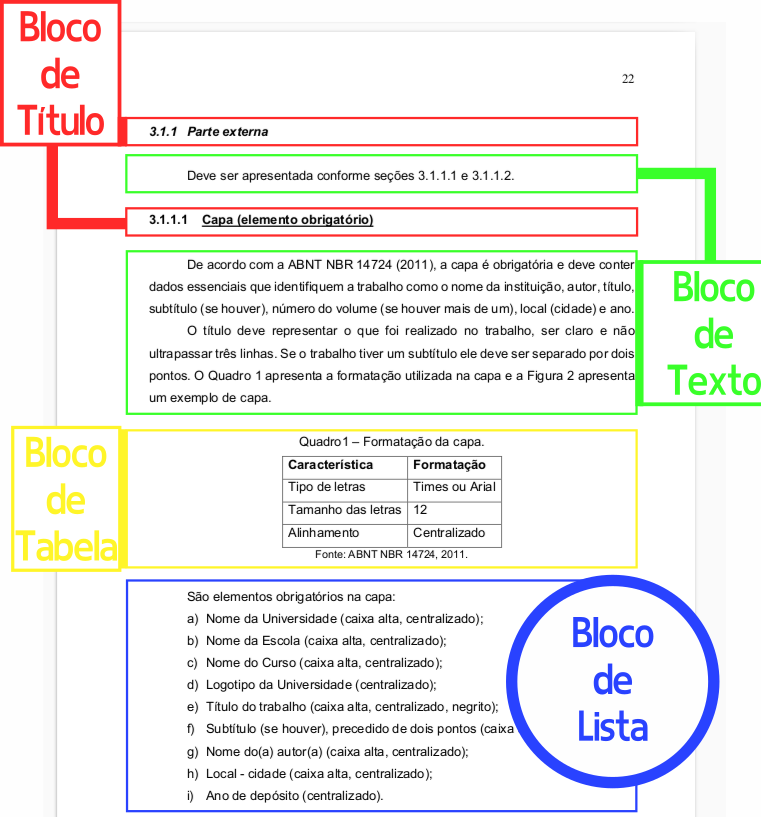
\includegraphics[width=0.8\textwidth]{./images/blocos-no-documento.png}
    \label{fig:blocos-no-documento} \\
    \textnormal{\fontsize{10pt}{12pt}Fonte: Adaptado de \cite{pucgo}}
\end{figure}

\subsection{Parsing}

O processo de Parsing é o processo que acontecerá sempre que o usuário desejar
ver o
\textit{layout}\footnote{
Do inglês: Disposição, ou esboço. Esta palavra geralmente está associada ao desenho ou visual de algo.
}
da versão final de seu trabalho. Ele usa o código intermediário gerado pelos blocos para montar o
\acrshort{pdf}
final.

Este processo é, em termos simples, uma espécie de análise a ser aplicada no código gerado pelos blocos
da aplicação. A plataforma gerará um código
\acrshort{json}\footnote{
Ver (sessão que trata do JSON)
}
como resultado das interações do usuário, que posteriormente
serão convertidos em código
latex\footnote{
Ver (sessão que trata do latex)
}.
Só então, finalmente será utilizado um utilitário que converterá o código latex
em um documento
\acrshort{pdf}. A
Figura\ref{fig:app-json-latex-pdf} ilustra esse processo:

\begin{figure}[ht]
    \centering
    \caption{Etapas do processo de Parsing}
    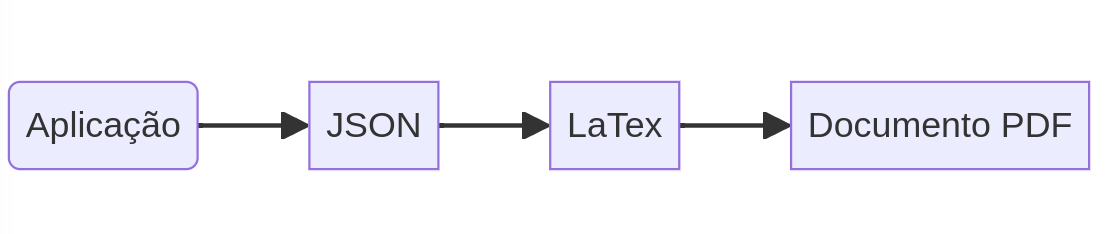
\includegraphics[width=0.9\textwidth]{./images/app-json-latex-pdf.png}
    \label{fig:app-json-latex-pdf} \\
    \textnormal{\fontsize{10pt}{12pt}Fonte: Autoria própria.}
\end{figure}

\section{Ambiente de desenvolvimento}

O ambiente de desenvolvimento é de extrema importância para que todas as ferramentas
utilizadas possam funcionar em perfeita harmonia em suas respectivas integrações e
colaborações. Muitas vezes, problemas de compatibilidade podem afetar
o funcionamento das mesmas e impedir que o programa final
seja executado corretamente, causando
\textit{bugs}\footnote{
Do inglês: Inseto. Esta palavra é muito utilizada no contexto de desenvolvimento de aplicativos
para se referir a problemas que afetam o funcionamento dos mesmos
}
e outros imprevistos impeditivos tanto para a correta execução, quanto
para a exeperiência de desenvolvimento.
A lista abaixo diz respeito às ferramentas e ao ambiente onde este \textit{software}
foi desenvolvido, bem como todas as suas respectivas versões:

\clearpage

\subsection{Lista de tecnologias do ambiente de desenvolvimento}

\begin{itemize}
        
	\item Npm 10.2.3
	\item Yarn 1.22.19
	\item NodeJs 20.10.0
	\item kpathsea version 6.3.4/dev
	\item Sistema Operacional: Ubuntu 20.04
	\item makeglossaries (Utilitário latex)
	\item BibTeX 0.99d (TeX Live 2022/dev/Debian)
	\item pdfTeX 3.141592653-2.6-1.40.22 (TeX Live 2022/dev/Debian)
    
\end{itemize}

\section{Resultados}

\chapter{Fundamentação teórica}